\section{Finding Cast Usage Patterns}
\label{sec:casts:methodology}

Since casts represent a problem for developers,
we aim to provide an answer for our research questions,
\ref{casts:rq1} (\emph{\crqA}),
\ref{casts:rq2} (\emph{\crqB}) and
\ref{casts:rq3} (\emph{\crqC}).
To answer them several elements are needed.
We need a corpus of representative ``real world'' code and we need to perform
source code analysis to identify cast operations and to help classify these
operations into usage patterns.


\subsection{Corpus Analysis}

We gathered cast usage data using the \ql{} query language,
``a declarative, object-oriented logic programming language for querying
complex, potentially recursive data structures encoded in a relational data
model''~\citep{avgustinovQLObjectorientedQueries2016}.
\ql{} allows us to analyse programs at the source code level.
\ql{} extracts the source code of a project into a Datalog model.
Besides providing structural data for programs, \ie{}, ASTs,
\ql{} has the ability to query static types and perform data-flow analysis.
To test our \ql{} queries,
we have used the \lgtm{} service provided by Semmle,%
\footnote{\url{https://lgtm.com/}}
the developers of \ql{}.
To gather all cast expressions used in this study,
we asked Semmle developers to run a query essentially like Query~\ref{lst:ql:all} on their entire database.

The \lgtm{} database includes---at the time of writing---7,559 \java{} projects imported from
open-source projects hosted in \github{}.
The \lgtm{} database was constructed by importing popular open-source projects, \eg{},
Apache Maven,\footnote{\url{https://lgtm.com/projects/g/apache/maven}}
Neo4j,\footnote{\url{https://lgtm.com/projects/g/neo4j/neo4j/}}, and
Hibernate\footnote{\url{https://lgtm.com/projects/g/hibernate/hibernate-orm/}}.
Additionally it includes projects exported by developers
to \lgtm{} to query them for bug finding, smell detection, and
other analyses.
We argue that this project selection provides a wide coverage over realistic
\java{} applications, excluding
uninteresting projects, \eg{}, student projects.

\subsection{Is the Cast Operator used?}

\newcommand{\nproject}{195}
\newcommand{\nloc}{19,264,590}
\newcommand{\nexpr}{57,292,018}
\newcommand{\nstmt}{13,270,506}
\newcommand{\nmethod}{1,492,490}
\newcommand{\nmethodwithcast}{99,018}
\newcommand{\castpercentage}{5.47}


\begin{figure}[ht!]
  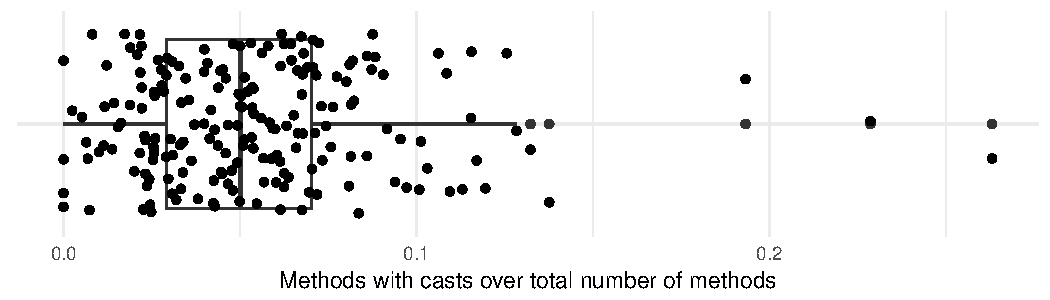
\includegraphics[width=\columnwidth]{analysis/stats-methodwcastXproject.pdf}
  \caption{Projects, by fraction of their methods containing casts. Bulk of data summarized by box plot, outliers shown as individual data points.}
  \label{fig:stats}
\end{figure}

We want to know how common cast usage is across projects (\ref{casts:rq1}).\footnote{
We collected the data for this section after completing our manual analysis of
casts (Section~\ref{sec:casts:methodology}).
Given that the \lgtm{} database is continuously evolving,
we were unable to analyze the exact same set of projects from which we had drawn our sample.
}
The box plot in Figure~\ref{fig:stats} shows, for each project,
the fraction of non-native non-abstract methods containing at least one cast.
The x-axis represents the fraction (1 means 100\% of methods contain casts).
The y-axis has no meaning and is just used to randomly spread the data
points for outliers.
For outliers, each dot represents a project,
and its size is given by the number of compilation units (C.U.) in the project.
There are projects where none of the methods contain a cast (at $x=0$),
but there are also four small projects
where all methods contain a cast (at $x=1$;
e.g., an SSL\,Ping tool implemented in a single method).
The plot shows that for most projects, fewer than a quarter of their
methods contain casts.
Overall, of the \nmethod{} non-abstract non-native methods in the database,
\nmethodwithcast{} (8.7\%) contained at least one cast.
The following sections analyze why there are cast instances (\ref{casts:rq2})
and how often the use cases that lead to casts occur (\ref{casts:rq3}).


\subsection{Manual Detection of Cast Patterns}

We initially sought to describe patterns precisely as \ql{} queries so that
detection and categorization was repeatable,
but we found this was infeasible because of the
complexity of the reasoning involved in identifying some patterns.
Often determining to which pattern a cast belongs requires reasoning about the run-time source of the cast,
which might be non-local and might depend on external application frameworks or generated code.
Thus, we resorted to manually inspect casts in order to devise cast usage patterns.

Nevertheless, whenever possible,
we provide a \ql{} query that \emph{approximates} the detection of some patterns.
That is, cast expressions returned as the result of a \ql{} query for a pattern,
most often belong to that pattern.
However, there could be other cast expressions not returned by the query,
which are instances of the pattern.
Our \ql{} queries used for pattern detection can be found online.%
\urlnote{https://gitlab.com/acuarica/java-cast-queries}

Unfortunately, we do not possess the \lgtm{} database.
It is not feasible for us to run our queries on their database.
Therefore, it is impractical to gather partial statistics using our queries.


\subsection{Methodology}

To identify patterns of cast usage, we analysed all \java{} projects in the \lgtm{} database, 7,559 projects
with a total 10,193,435 casts, at the time of writing.
There are 215 projects in the database for which we could not retrieve the source code.
In total, these 215 projects contain 1,162,583 casts.
Moreover, there are also 516 projects that do not contain any cast.
Therefore the total cast population to be analysed consists of 9,030,852 casts in 6,840 projects.

Because the number of cast instances is large, it is not feasible to \emph{manually} analyse all of them.
Therefore we have opted to perform random sampling to get a subset of cast instances to analyse.
To choose a sample size such that
the probability of missing the least frequent pattern is extremely low, we assume a
hypergeometric distribution of the data.
The hypergeometric distribution is a discrete probability distribution used with a finite population of $N$ subjects.
It is used to calculate the probability of drawing $k$ subjects with a given feature---provided that there are $K$ subjects with that feature in the population---in $n$ draws, without replacement.

Returning to our problem of finding an appropriate sample size, we model our question as follows:
We assume there are $K$ casts that are members of the least frequently occurring pattern.
We want to know the probability of not finding this pattern, \ie, sampling exactly $k = 0$.
Our population consists of $N = 9,030,852$ cast instances.
For our study, we assume that a pattern is irrelevant if it represents less than $0.1\%$ of the population, or $K = 9,031$ cast instances.
Plugging-in these parameters using the hypergeometric distribution formula,%
\footnote{The reader can use any hypergeometric distribution calculator, \eg{}, \url{https://keisan.casio.com/exec/system/1180573201}}
we found that with a sample size of $n = 5,000$ the probability of not sampling the
least frequently occurring pattern is $0.67\%$.

\begin{figure}[ht!]
  \includegraphics[width=\columnwidth]{analysis/dist-all-log.pdf}
  \caption{Cast distribution}
  \label{fig:dist}
\end{figure}

Our sample represents a set of casts coming from various projects in the database.
We sampled 5000 casts, but there are more than 5000 projects in the database,
so not every project is represented in our sample.
Figure~\ref{fig:dist} compares the projects in the database
to the projects from which we sampled at least one cast.
The x-axis shows the number of casts in a project,
the y-axis shows the fraction of projects with fewer than x casts.
In the population, 50\% of projects have fewer than 100 casts,
but in the sample, only 6\% of projects have fewer than 100 casts.
Our sample is thus somewhat biased towards larger projects,
which is to be expected, given that projects with more casts
had a larger probability to be sampled.
Remember, we sampled casts, not projects.
Nevertheless, the sample does include projects across the entire spectrum,
with 50\% of projects having fewer than 2,000 casts.

\newcommand\col[1]{\textsf{#1}}
The manual categorization file can be found online.%
\footnote{\url{https://gitlab.com/acuarica/phd-thesis/blob/master/analysis/casts.csv}}
This file is a comma-separated values (CSV) table.
Each row represents a cast instance.
This table contains 6 columns.
The \col{castid} and \col{repoid} columns represent internal IDs to uniquely identify each cast instance and each project.
The \col{target} and \col{source} columns indicate the source and target types used in the cast.
The last two columns---\col{link} and \col{value}---are the link to the source code file in \lgtm{} and the result of the manual inspection.
The script to process the results of the manual inspection is available online as well.%
\footnote{\url{https://gitlab.com/acuarica/phd-thesis/blob/master/analysis/analysis.r}}
We had to sample more than \nSize{} casts.
The CSV table mentioned above contains \nSeen{} casts (rows).
This is because we found \nBrokenLink{} links that were not accessible during our analysis,
making manual code inspection impossible.
Inaccessible links can be found because some projects were removed from the \lgtm{} platform.
We also found \nBug{} cast that was clearly a bug,
a downcast using the wrong cast operand.
Thus, we had to resample the cast instances until we reach \nSize{} manually inspected casts.
When resampling, we took care of inspecting \emph{different} cast instances, \ie{},
we have discarded duplicated casts.
We found \nDuplicated{} duplicated casts when resampling.
